
\chapter{Implementierungsprobleme}

In den bisherigen Kapiteln haben wir das Thema "`Sicherheit"' hauptsächlich aus einem kryptographischen Blickwinkel betrachtet und eine Vielzahl von kryptographischen Primitiven vorgestellt.

In diesem Kapitel wollen wir uns nun mit einer anderen Seite der Sicherheit befassen: Der Sicherheit bzw. Unsicherheit von Software. Wir betrachten Sicherheitslücken in Software, wie sie täglich von Computerviren und Ähnlichem ausgenutzt werden. Solche Sicherheitslücken entstehen fast immer durch kleine oder große Schlampereien bei der Implementierung.

Die "`Common Vulnerabilites and Exposures"' (CVE) ist eine öffentlich zugängliche Liste bekannter Schwachstellen.
Sie ist unter \url{http://cve.mitre.org/cve/} erreichbar, und zählte im Dezember 2013 knapp 60.000 Einträge.
Die amerikanische "`National Vulnerabilities Database"' (NVD, \url{http://nvd.nist.gov/}) des "`National Institute for Standards and Technology"' (NIST) bietet eine Suchfunktion in dieser Datenbank, inklusive einfacher statistischer Anfragen.
Das "`Open Web Application Security Project"' (OWASP, \url{https://www.owasp.org/}) erstellt alle drei Jahre eine Top-Ten-Liste der Sicherheitslücken in Web-Anwendungen.

Wir stellen im Folgenden einige übliche Angriffstechniken von Hackern auf anfällige Software vor. Wir werden uns jedoch auch kurz mit Implementierungsproblemen von kryptographischen Operationen befassen.

\section{Buffer Overflows}

In einigen Programmiersprachen (allen voran C und C++) erfolgen Zugriffe auf Puffer (oder Arrays/Felder) ohne eine Überprüfung der Größe der Puffer. Z.B. liefert folgendes C-Programm keinen Fehler:

 %Das Uchanges Paket und das Listings-Paket scheinen zusammen nicht toll zu funktionieren.

\begin{lstlisting}
	#include <stdio.h>
	
	char greeting[8] = "Hello, ";
	char greeted[6] = "World";
	
	int main() {
		printf("%c\n", greeting[8]);
		return 0;
	}
\end{lstlisting}


Dabei hat in diesem Beispiel das Feld \lstinline+greeting+ nur 8 Elemente, die von 0 bis 7 durchnummeriert sind.%
\footnote{In C erhalten Strings immer noch ein terminierendes Null-Symbol $\backslash$0, das das Ende des Strings markiert. Deshalb benötigt die Zeichenkette \lstinline[showspaces=true]+Hello,\ +, die aus sieben Zeichen besteht, dennoch 8 Byte Speicherplatz. Analog benötigt die Zeichenkette \lstinline+World+ (5 Zeichen) 6 Byte.}
Ein Zugriff auf das Element mit der Nummer 8 ist also eigentlich nicht möglich, die Rückgabe bestenfalls undefiniert.
Dennoch löst das Programm keinen Fehler aus, sondern gibt den Buchstaben "`W"' aus.\footnote{Kompiliert mit GCC 4.6.1}\\

Dies liegt an der Implementierung von Puffern in C:
Ein Puffer oder Feld ist in C äquivalent zu einem Zeiger auf das erste Pufferelement (Index 0).
Die Elemente des Puffers sind dann unmittelbar hintereinander angeordnet.
Um die Speicheradresse des $i$-ten Elements (Index $i - 1$) zu bestimmen, wird daher der Platzbedarf der vorherigen $i-1$ Elemente berechnet und dieser Wert zur Startadresse des Puffers hinzuaddiert.
Diese Berechnung erfolgt im Allgemeinen ohne Abgleich mit der Größe des Puffers.

Im obigen Beispiel ist \lstinline+greeting+ im Wesentlichen ein Zeiger auf einen Speicherbereich, in dem die Zeichen \lstinline+Hello, + hintereinander abgelegt sind.
Der Zugriff auf \lstinline+greeting[8]+ erfolgt, in dem der Platzbedarf von 8 \lstinline+char+s zum Zeiger \lstinline+greeting+ hinzuaddiert werden.

Da der Compiler in diesem Beispiel die beiden Speicherbereiche für die Zeichenketten \lstinline+Hello, + und \lstinline+World+ hintereinander angeordnet hat,
liegt 8 Positionen hinter dem Speicherbereich \lstinline+greeting+ der Buchstabe \lstinline+W+ aus der Zeichenkette \lstinline+World+.
Das Speicherlayout wird in Abbildung \ref{fig:impl:memorylayoutexample} gezeigt.

\begin{figure}[h]
	\begin{center}
		\setlength{\unitlength}{0.8mm}
		\begin{picture}(160,50)(-10,-20)
			%the grid
			\put(0,0){\line(1,0){140}}
			\put(0,10){\line(1,0){140}}
			\multiput(0,0)(10,0){15}{\line(0,1){10}}
			
			%the content, namely the strings
			\put(  4,3){H}
			\put( 14,3){e}
			\put( 24,3){l}
			\put( 34,3){l}
			\put( 44,3){o}
			\put( 54,3){,}
			\put( 64,3){ }
			\put( 72,3){$\backslash$ 0}
			\put( 83,3){W}
			\put( 94,3){o}
			\put(104,3){r}
			\put(114,3){l}
			\put(124,3){d}
			\put(132,3){$\backslash$ 0}
			
			%the arrows and markers
			\put(  5,-10){\vector(0,1){10}}
			\put(  1,-15){\lstinline+greeting+}
			\put( 85,-10){\vector(0,1){10}}
			\put( 85,-15){\lstinline+greeted+}
			
			\put( 25, 20){\vector(0,-1){10}}
			\put( 20, 22){\lstinline+greeting[2]+}
			\put( 85, 20){\vector(0,-1){10}}
			\put( 80, 22){\lstinline!greeting[8]!}
		\end{picture}
	\end{center}
	\caption{Anordnung der zwei Speicherbereiche \lstinline+greeting+ und \lstinline+greeted+ in unserem Beispiel. Ein Zugriff auf \lstinline+greeting[8]+ addiert den Speicherplatzbedarf von 8 \lstinline+char+s zu dem Zeiger \lstinline+greeting+. Beim Zugriff wird deshalb tatsächlich auf \lstinline+greeted[0]+ zugegriffen.}
	\label{fig:impl:memorylayoutexample}
\end{figure}

Ein Schreibzugriff auf \lstinline+greeting[8]+ liefert in diesem Beispiel ebenfalls keinen Fehler, selbiges gilt Schreibzugriffe auf \lstinline+greeting[9]+, \lstinline+greeting[10]+, usw. bis zumindest \lstinline+greeting[12]+.

Dieses Verhalten führt dazu, dass ganze Speicherbereiche überschrieben werden.
Wir betrachten hierzu das folgende Beispiel:


\begin{lstlisting}[firstline=3]
#include <stdio.h>

char name[8] = "World";
char greeting[8] = "Hello, ";

int main() {
	printf("What's your name?\n");
	scanf("%s", name);
	printf("%s%s\n", greeting, name);
	return 0;
}
\end{lstlisting}


Dieses Programm liest zunächst den Namen des Benutzers mittels der Funktion \lstinline+scanf+ in den Speicherbereich \lstinline+name+ ein,
und gibt dann die zwei Strings \lstinline+greeting+ und \lstinline+name+ aus.
Ist der Name des Benutzers jedoch länger als 7 Zeichen,
dann überschreibt die Funktion \lstinline+scanf+ nicht nur den Speicherbereich der Variable \lstinline+name+,
sondern auch den Speicherbereich des Strings \lstinline+greeting+.
	
Im Allgemeinen wird die Funktion \lstinline+scanf+ so viel Speicherplatz überschreiben,
wie sie zum Speichern der eingegebenen Daten benötigt.
Bietet der bereitgestellte Puffer nicht genug Speicherplatz,
so wird \lstinline+scanf+ auf den dahinterliegenden Speicherbereich zugreifen und diesen überschreiben.%
\footnote{Selbiges gilt für eine Vielzahl anderer Funktionen in C, z.B. \lstinline+strcat+ zum Konkatenieren von zwei Strings, \lstinline+strcpy+ zum Kopieren von Strings, uvm.}
Der Puffer "`läuft also über"'. Man bezeichnet so etwas deshalb als "`Buffer Overflow"'.

Dieses unerwünschte Verhalten kann ein Angreifer ausnutzen um gezielt bestimmte Daten im Arbeitsspeicher des ausgeführten Programms zu überschreiben.
Befindet sich der übergelaufene Puffer auf dem Stack des Programms,
dann kann der Angreifer mit dieser Technik sogar die Rücksprungadresse überschreiben und somit den Programmfluss lenken.

Hat der Angreifer zuvor eigenen Maschinencode (d.h. Prozessorinstruktionen) in den Arbeitsspeicher des Programms geschrieben,
dann kann der Angreifer somit eigenen Programmcode auf dem Prozessor ausführen lassen.\\

Da diese Angriffstechnik über Jahre hinweg genutzt wurde, wurden inzwischen eine ganze Reihe von Gegenmaßnahmen entwickelt. Im Folgenden wollen wir einige dieser Gegenmaßnahmen vorstellen.%
\footnote{Es gibt aber zahlreiche Abwandlungen des gezeigten Angriffs, die diese Schutzmaßnahmen umgehen und deshalb auch heute noch funktionsfähig sind.}

Eine offensichtliche Gegenmaßnahme ist das vollständige Verhindern von Buffer Overflows.
Hierzu kann man z.B.:
\begin{itemize}
	\item vor jedem Schreibzugriff auf einen Puffer explizit die Puffergröße kontrollieren,
	\item Funktionen benutzen, die diese Kontrolle automatisch durchführen, (z.B. \lstinline+strncat+ oder \lstinline+strncpy+; bei \lstinline+scanf+ kann man in obigem Beispiel \lstinline+scanf("\%7s", name)+ verwenden), oder
	\item eine Datenstruktur oder Programmiersprache verwenden, die beim Zugriff auf Puffer automatisch die Grenzen überprüft (z.B. Arrays in Java).
\end{itemize}

Da die erste Methode sehr anfällig für menschliche Vergesslichkeit oder Bequemlichkeit ist, sind die zweite oder dritte Maßnahme hier eindeutig vorzuziehen.\

Diese Gegenmaßnahmen sind jedoch nicht immer anwendbar.
Z.B. existieren einige weit verbreitete und sehr umfangreiche Programme mit mehreren Millionen Zeilen Quellcode, die noch ohne derartige Gegenmaßnahmen implementiert wurden.
Den Quellcode dieser Programme zu überarbeiten ist praktisch kaum umsetzbar.
Deshalb wurden auch eine Reihe von ad-hoc-Gegenmaßnahmen entwickelt.
Hierzu zählen Stack Canaries, die sogenannte Data Execution Prevention und die Address Space Layout Randomization.\\

Stack Canaries werden von modernen Compilern in den generierten Maschinencode eingebettet.
Hierbei handelt es sich um zufällige Dummy-Zahlen, die vor Rücksprungadressen auf dem Stack platziert werden.
Tritt ein Buffer Overflow auf bei dem die Rücksprungadresse überschrieben wird, so muss dieser Buffer Overflow auch den Stack Canary, der zwischen Puffer und Rücksprungadresse liegt, überschreiben.

Der Compiler fügt vor jedem Rücksprung im generierten Code noch einige Befehle ein, die überprüfen ob der Stack Canary verändert wurde.
Ist dies der Fall, so wird das Programm beendet.
Ist der Stack Canary unverändert, so geht das Programm davon aus, dass kein Buffer Overflow auftrat und setzt die Ausführung fort.\\

Bei der Data Execution Prevention, die vom Prozessor unterstützt und vom Betriebssystem aktiviert werden muss,
erzwingt der Prozessor eine Trennung von Code- und Speicherbereichen.
Daten in Speicherbereichen können dann nicht als Programmcode interpretiert werden, und Daten in Code-Bereichen können nicht überschrieben werden.
Dadurch kann der Angreifer den von ihm eingeschleusten Code nicht ausführen lassen.\\

Bei der Address Space Layout Randomization (auch als Speicherverwürfelung bezeichnet) platziert das Betriebssystem die Speicherbereiche des Programms nicht deterministisch, sondern zufällig.
Um den eingeschleusten Code auszuführen, muss der Angreifer nämlich die Rücksprungadresse auf dem Stack mit der Adresse des eingeschleusten Codes überschreiben.
Wegen der zufälligen Platzierung der Speicherbereiche kann der Angreifer diese Adresse jedoch nicht kennen.


\section{SQL-Injection}

SQL ist eine weit verbreitete Sprache zur Formulierung von Datenbankabfragen. Zum Beispiel bewirkt die Abfrage
\begin{lstlisting}[language=SQL]
  SELECT * FROM cd WHERE interpret = "Fall Out Boy";
\end{lstlisting}

die Rückgabe aller Zeilen in der Tabelle \lstinline+cd+, in denen als Interpret "`Fall Out Boy"' angegeben ist.
Nun könnte diese Tabelle in einer Datenbank eines Online-Musikshops liegen. Dieser Online-Musikshop bietet dem Nutzer eine Suchfunktion.
Sucht der Nutzer nach CDs von "`Fall Out Boy"', dann wird z.B. obige Anfrage an die Datenbank geschickt.
Sucht der Nutzer stattdessen nach dem Album "`Folie \`a Deux"', so wird stattdessen die Anfrage 

\begin{lstlisting}[language=SQL,escapechar=+]
  SELECT * FROM cd WHERE album = "Folie +\ttfamily \`a+ Deux";
\end{lstlisting}

an die Datenbank geschickt.

Eine naheliegende Implementierung zur Generierung solcher Datenbankabfragen in der Programmiersprache PHP ist z.B. Folgende.

\begin{lstlisting}[language=PHP]
  $alb = $_GET['album'];
  sql_query($db,"SELECT * FROM cd WHERE album = \"$alb\";");
\end{lstlisting}
\label{listing:impl:SqlInjectionInPhp}

Hierbei enthält die Variable \lstinline+$_GET['album']+ die Benutzereingabe. Diese wird zunächst in die Variable \lstinline+$alb+ kopiert. Der String

\begin{lstlisting}[language=PHP]
	"SELECT * FROM cd WHERE album = \"$alb\";"
\end{lstlisting}

wird automatisch in eine Konkatenation des Strings "`\lstinline+SELECT * FROM cd WHERE album = "+"', dem Inhalt von \lstinline+$alb+  und des Strings "`\lstinline+ \";+"' umgesetzt.
Das Ergebnis dieser Konkatenation wird dann durch die Funktion \lstinline+sql_query+ als Abfrage an die Datenbank geschickt.\\

Leider erlaubte diese einfache Implementierung einem Angreifer, selbst festgelegte Befehle an die Datenbank zu senden. Hierfür muss er nur -- anstelle eines Albums -- Strings wie "`\lstinline+\"; DROP TABLE cd; #+"' in die Suchmaske eingeben.

Die Stringkonkatenation führt dann zur Abfrage
\begin{equation*}
	\underbrace{\texttt{SELECT * FROM cd WHERE album = \dq}}_{\mathrm{Konstant}}
	\underbrace{\texttt{\dq; DROP TABLE cd; \#}}_{\mathrm{Benutzereingabe}}
	\underbrace{\text{\ttfamily "\phantom{"};}}_{\mathrm{Konstant}} \text{, }
\end{equation*}
die an die Datenbank geschickt wird. Die Datenbank interpretiert diese Abfrage als zwei Anweisungen:%
\footnote{Das \#-Symbol leitet einen Kommentar ein. Dadurch wird verhindert, dass die folgenden Zeichen "`\lstinline+\";+"' einen Syntaxfehler auslösen.}
\begin{enumerate}
	\item die Suche nach Alben, deren Name das leere Wort ist, und
	\item die Anweisung, die Tabelle "`\lstinline+cd+"' zu löschen.
\end{enumerate}
Beide Anweisungen werden von der Datenbank ausgeführt, und so wird die Tabelle "`\lstinline+cd+"' tatsächlich gelöscht. Der Angreifer hat also eigene Befehle in die Datenbankabfrage "`injiziert"', daher rührt die Bezeichnung "`SQL-Injection"' für solche Sicherheitslücken.

SQL-Injection-Angriffe können aber noch ungleich gefährlicher werden, wenn die Software besondere Funktionen wie das Ausführen von Kommandozeilenbefehlen oder das Erstellen von Dateien erlaubt.
Ersteres ist z.B. bei Microsoft-SQL-Servern der Fall, Letzteres z.B. bei MySQL-Servern.\\

Solche Angriffe kann man z.B. mit den folgenden Methoden verhindern:
\begin{itemize}
	\item Gründliche Überprüfung der Benutzereingabe, bevor diese an die Datenbank geschickt wird.
	Sinnvoll wäre z.B. eine Überprüfung, ob die Benutzereingabe nur aus Buchstaben, Zahlen und Leerzeichen besteht.
	(Dies kann allerdings unnötig restriktiv sein. Z.B. könnte die Eingabe des Zeichens \`a dadurch zurückgewiesen werden, obwohl es ein Album mit einem solchen Namen gibt.)
	\item Das "`Escapen"' von Sonderzeichen in der Benutzereingabe, so dass diese als Bestandteil des Strings interpretiert werden.
	Hierfür gibt es in den APIs der Datenbank häufig besondere Funktionen, z.B. \lstinline+mysql_real_escape_string+.
	\item Das Benutzen von Prepared Statements. Hierbei wird zunächst ein Abfrage mit Platzhalter an die Datenbank geschickt:
\lstinline+SELECT * FROM cd WHERE album=?;+
	In einem zweiten Schritt wird dann die Benutzereingabe an die Datenbank übergeben.
	Hierdurch wird verhindert, dass die Benutzereingabe von der Datenbank als Befehl interpretiert und ausgeführt wird.
\end{itemize}

\section{Cross Site Scripting}

Cross-Site-Scripting (XSS) funktioniert konzeptuell ähnlich wie SQL-Injections, taucht jedoch in einer etwas anderen Umgebung auf.\\

Bei Cross-Site-Scripting injiziert ein Angreifer nicht eigene SQL-Befehle in eine Datenbankabfrage,
sondern stattdessen eigene HTML-Elemente in eine Webseite.
Über JavaScript im injizierten HTML kann die im Browser des Opfers dargestellte Webseite vollständig kontrolliert werden, was
ernsthafte Konsequenzen zur Folge haben kann.
\begin{itemize}
	\item Gelingt es dem Angreifer beispielsweise eigenen JavaScript-Code auf einer Login-Seite zu platzieren, so kann der Angreifer hiermit die von einem Opfer eingegebenen Login-Daten abgreifen.
Doch auch wenn ein Benutzer bereits eingeloggt ist, kann der Angreifer mit entsprechendem JavaScript-Code das Login-Cookie des Benutzers kopieren und damit selbst unter der Identität des Nutzers auf der Webseite surfen.
	\item JavaScript-Würmer können in sozialen Netzwerken auf Pinnwände oder Ähnliches geschrieben werden, wo sie von anderen Benutzern eingesehen werden. Sie werden daraufhin im Browser des Opfers ausgeführt und kopieren sich selbstständig auf die Pinnwand des Betrachters.
Beispielsweise wurde MySpace im Jahr 2005 zeitweilig wegen einem solchen Wurm abgeschaltet.\cite{Kamkar2005, Sophos}.
	\item Die Computer-Forensik-Software X-Way Forensics bietet z.B. die Möglichkeit, ihre Ergebnisse als HTML-Seite darzustellen.
Bettet ein Angreifer z.B. einen öffnenden HTML-Kommentar in die Windows-Registry-Key ein, und einen schließenden Kommentar in einen späteren Registry-Key, dann werden die dazwischen liegenden Registry-Keys dem Nutzer nicht angezeigt.
Diese Sicherheitslücke wurde 2011 bekannt und behoben \cite{Wundram2011}.
	\item Cross-Site-Scripting kann auch als Implementierung für den CRIME-Angriff auf TLS verwendet werden (siehe Kapitel \ref{sec:keyex:crime}).
\end{itemize}

Eine typische Gegenmaßnahme gegen XSS-Angriffe ist es, von Benutzern stammende Daten entsprechend zu maskieren, damit sie vom Browser nicht als HTML interpretiert werden können.
Die Programmiersprache PHP bietet hierfür z.B. die Funktionen \lstinline+htmlspecialchars+ und \lstinline+htmlentities+, die Zeichen mit spezieller Bedeutung in HTML (z.B. \lstinline+<+, \lstinline+>+, und \lstinline+\"+) ersetzen.

\section{Denial of Service}

Denial of Service (DOS) Angriffe zielen, anders als die bisher vorgestellten Angriffe, nicht darauf ab, selbstbestimmten Code auf einem fremden Server ausführen zu lassen.
Ziel ist es bei solchen Angriffen nur einen bestimmten Dienst lahmzulegen, z.B. das Online-Banking einer Bank oder einen Onlineshop.
Bei solchen Angriffen handelt es sich jedoch nicht immer nur um digitalen Vandalismus.

In einigen Fällen versuchten Kriminelle mit solchen Angriffen z.B. Geld von Onlineshops zu erpressen.
Die Gruppe Anonymous protestierte auf diese Art auch dagegen, dass einige Banken Spenden an Wikileaks nicht mehr ausführten.\\

\subsection{DDOS}

Eine technisch einfache Möglichkeit für DOS-Angriffe ist es, den Server, der den Dienst erbringt, mit Anfragen zu überhäufen. Dann kann der Server nämlich aufgrund seiner beschränkten Ressourcen nur einen kleinen Teil der Anfragen bearbeiten, so dass der Service für die eigentlichen Nutzer effektiv nicht mehr zur Verfügung steht.

Je nach Ausstattung des Servers werden dabei die Datenleitungen zum Server überlastet, das Betriebssystem des Servers, dass die Netzwerkverbindungen verwalten muss, oder der Prozessor des Servers, der für die Bearbeitung der Anfragen Rechenleistung erbringen muss.

Im Allgemeinen werden für eine solche Überlastung jedoch eine ganze Reihe von Angreifern benötigt, die gemeinsam versuchen den Server zu überlasten.
Deshalb werden solche Angriffe auch als "`Distributed Denial Of Service"'-Angriffe (DDOS-Angriffe) bezeichnet.
In der Realität werden solche Angriffe üblicherweise durch Bot-Netze ausgeführt.
Ein Botnetz ist ein Netzwerk von mit Viren oder anderer Schadsoftware infizierter Computer.
Auf den Befehl des Autors der Schadsoftware hin führen diese bestimmte Aufgaben aus, z.B. eben eine DDOS-Attacke auf ein bestimmtes Ziel.\\

Eine Variante von solchen DDOS-Angriffen, die darauf abzielt, die Verwaltung von Netzwerkverbindungen durch das Betriebssystem zu überlasten, ist das sogenannte "`SYN-Flooding"'.
SYN-Pakete werden verwendet, um TCP-Verbindungen aufzubauen.
Erhält ein Server ein SYN-Paket mit einer bestimmten Sequenznummer, und möchte der Server die Verbindung akzeptieren, so antwortet er auf das SYN-Paket mit einem SYN+ACK-Paket und einer eigenen Sequenznummer. Unterdessen speichert er einige Informationen zur noch nicht vollständig aufgebauten Verbindung, z.B. die IP-Adresse des Clients, den vom Client verwendeten TCP-Port und die selbst vergebene Sequenznummer.
Bei einem normalen Verbindungsaufbau antwortet der Client dann noch einmal mit einem "`ACK"'-Paket, um den Aufbau der TCP-Verbindung abzuschließen. Abbildung \ref{fig:impl:TcpHandshake} zeigt ein Beispiel eines normalen TCP-Verbindungsaufbaus.

\begin{figure}[htbp]
	\begin{center}
		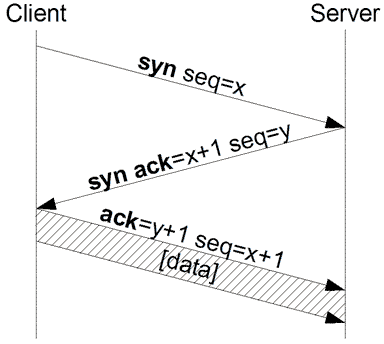
\includegraphics[scale=0.5]{images/300px-Tcp-handshake.png}
	\end{center}
	\caption{Beispiel eines TCP-Verbindungsaufbaus. Quelle: http://commons.wikimedia.org/wiki/File:300px-Tcp-handshake.png Lizenz: CC-BY-SA 3.0 Unported Autor: vermutlich Caos}
	\label{fig:impl:TcpHandshake}
\end{figure}

Beim SYN-Flooding jedoch sendet der Client niemals das abschließende ACK-Paket, sondern sendet weitere SYN-Pakete um noch mehr TCP-Verbindungen aufzubauen.
Dadurch zwingt der Angreifer den Server dazu, Informationen zu jeder noch nicht vollständig aufgebauten Verbindung zu speichern.
Da der zur Verfügung stehende Speicherplatz jedoch beschränkt ist, lässt sich damit die Verwaltung der Netzwerkverbindungen im Betriebssystem belasten. Arbeiten mehrere Angreifer zusammen, so kann man den Server hiermit überlasten.

\section{Andere DOS-Angriffe}

DDOS-Angriffe sind jedoch nicht die einzige Möglichkeit, einen Server lahmzulegen. Wir betrachten nun noch einen anderen beispielhaften Angriff, der technisch etwas interessanter ist.\\

Einige Sprachen, wie z.B. PHP, Python und JavaScript bieten die Möglichkeit Strings als Indizes von Arrays zu verwenden.
Wir haben dies bereits in unserem Beispiel zu SQL-Injection auf Seite \ref{listing:impl:SqlInjectionInPhp} gesehen. Dort wurde auf das (vordefinierte) Array \lstinline+$_GET+ zugegriffen. Dieses Array wird von PHP automatisch mit allen Parametern gefüllt, die der Client dem Server beim Aufruf einer Webseite per \lstinline+GET+-Methode übergibt. Z.B. wird bei der Anfrage
\begin{lstlisting}
http://www.example.com/?q=mad+magazine
\end{lstlisting}

der Wert "`\lstinline+mad magazine+"' unter dem Schlüssel "`\lstinline+q+"' in das (vordefinierte) Array \lstinline+$_GET+ eingefügt. Es ist also \lstinline+$_GET['q'] == 'mad magazine'+.

Intern wird hierfür eine Dictionary-Datenstruktur bzw. eine Hashtabelle verwendet.
Solchen Datenstrukturen liegt ein gewöhnliches (mit Zahlen indiziertes) Array $\overline{\texttt{\$\_GET}}$ der Länge $l$ sowie eine Hashfunktion $h$ zugrunde.
Um einen Wert $v_1$ (z.B. "'\lstinline+mad magazine+"') unter einem Index (oder Schlüssel) $s_1$ (z.B. "`\lstinline+q+"') zu speichern, wird der Schlüssel $s_1$ zunächst zu $h(s_1)$ gehasht.
Das Ergebnis wird modulo $l$ reduziert, und das Paar $(s_1, v_1)$ an der Position $h(s_1) \mod l$ im Array gespeichert.

Die Hashfunktion $h$ bietet jedoch keine kryptographische Kollisionsresistenz, da kryptographische Hashfunktionen zu aufwendig auszuwerten sind.
Deshalb kann es vorkommen, dass für ein zweites Schlüssel-Wert-Paar $(s_2, v_2)$ gilt, dass $h(s_2) \equiv h(s_1) \pmod l$ ist.
In diesem Fall müssen beide Paare $(s_1,v_1)$ und $(s_2,v_2)$ an der selben Stelle im Array gespeichert werden. Deshalb werden beide Paare üblicherweise in eine verkettete Liste eingefügt, die dann an dieser Stelle im Array $\overline{\texttt{\$\_GET}}$ gespeichert wird.%
\footnote{Eine Andere Strategie ist, $(s_2,v_2)$ an der nachfolgenden Stelle im Array zu speichern, sofern diese frei ist.}
Werden weitere Paare $(s_3, v_3), \ldots)$ mit $h(s_3) \equiv h(s_2) \pmod l$, \ldots, so werden diese Paare ebenfalls in die verkettete Liste eingefügt.\\

Tritt keine Hashkollision auf, so benötigt man für $n$ Zugriffe auf eine solche Dictionary-Struktur nur $\mathcal{O}(n)$ Operationen. Treten jedoch \emph{nur} Kollisionen auf, d.h. für alle $i,j$ gilt $h(s_i) \mod l = h(s_j) \mod l$, dann werden alle Elemente der Datenstruktur in \emph{nur einer} verketteten Liste gespeichert. Für $n$ Zugriffe werden dann $\Omega(n^2)$ Operationen benötigt.\\

Dies kann sich ein Angreifer zunutze machen. Da $h$ keine kryptographische Kollisionsresistenz bietet, kann der Angreifer eine große Anzahl entsprechender Schlüssel erzeugen, so dass diese in der Dictionary-Struktur des Servers alle in der selben Liste gespeichert werden. Dadurch kann der Angreifer gezielt eine hohe Last auf dem Server erzeugen.

Weitere Informationen zu diesem Angriff finden sich im Vortrag \cite{Klink2011}.
